\chapter{Main Results}
\label{chap:main}

\section{Degree Distance Index of Monocyclic Graph $C_k(s,t)$}
In this section, the study will show us how to derive the Degree distance index of the monocyclic graph $C_k(s,t)$. This will be done using Theorem \href{chap2.tex}{\ref{sec:dd_wiener}}.
$$ 
DD(C_k(s,t))=\sum_{u\in V(C_k(s,t))} w(u,C_k(s,t))deg(u)
$$

\begin{thm}\rm
$$DD(C_k(s,t))=\sum_{u\in G_s} dd(u,C_k(s,t))+\sum_{u\in G_k} dd(u,C_k(s,t))+\sum_{u\in G_t} dd(u,C_k(s,t))$$
\label{thm:degree_dist_u}
\end{thm}

\proof
Suppose we partition the vertex set of $C_k(s,t)$ into the following sets:
\begin{enumerate}
\item $G_s=\left\lbrace u_1,u_2,\cdots,u_s \right\rbrace$, the set containing $s$ pendant vertices.
\item $G_k=\left\lbrace v_1,v_2,\cdots,v_k \right\rbrace$ the set containing the vertices of the cycle $C_k$, where $v_1$ is attached with $s$ pendant vertices and $v_k$ is attached with $t$ pendant vertices.
\item $G_t=\left\lbrace w_1,w_2,\cdots,w_t \right\rbrace$ the set containing $t$ pendant vertices. 
\end{enumerate}
Now, the expanded form of the degree distance index of $C_k(s,t)$ is
\begin{equation}
DD(C_k(s,t))=\sum_{u\in G_s} w(u,C_k(s,t))deg(u)+\sum_{u\in G_k} w(u,C_k(s,t))deg(u)+\sum_{u\in G_t} w(u,C_k(s,t))deg(u)
\label{eqn:DD_part}
\end{equation}
note that the degree distance index of $C_k(s,t)$ at vertex $u$ is \medskip
\begin{equation}
dd(u,C_k(s,t))=w(u,C_k(s,t))deg(u)
\label{eqn:dd_u}
\end{equation}\\
thus, $DD(C_k(s,t))=\sum_{u\in G_s} dd(u,C_k(s,t))+\sum_{u\in G_k} dd(u,C_k(s,t))+\sum_{u\in G_t} dd(u,C_k(s,t))$ \qed

\begin{thm}\rm
The degree distance index of $C_k(s,t)$ at vertex $v_1$ is 
\begin{equation}
dd(v_1,C_k(s,t))=(s+2)(w(v_1,C_k)+s+2t) \label{eqn:dd_v1}
\end{equation}
and the degree distance index of $C_k(s,t)$ at vertex $v_k$ is 
\begin{equation}
dd(v_k,C_k(s,t))=(t+2)(w(v_k,C_k)+2s+t) \label{eqn:dd_vk}
\end{equation}
where $$w(v_1,C_k)=w(v_k,C_k)=\left\lbrace\begin{array}{cc}
\frac{k^2}{4} & $if k is even \\ 
\frac{(k+1)(k-1)}{4} & $if k is odd
\end{array}
$$
\label{thm:dd_v_1_k}
\end{thm}

\proof
Since $v_1$ and $v_k$ are vertices in the cycle $C_k$, then $deg(v_1)=(s+2)$, where $s$ is the number of pendant vertices attached to $v_1$ and $deg(v_k)=t+2$, where $t$ is the number of pendant vertices attached to $v_k$. 

Now, let us find $w(v_1,C_k(s,t))$. Using Lemma \href{chap2.tex}{\ref{sec:lem_wiener_u}} $v_1$ would be paired by the vertices at sets $G_s,G_k,G_t$ excluding itself. Computing their distances we have \medskip

\begin{enumerate}
\item {For all $u\in G_s$, the distance $d(v_1,u)=1$. Since there are $s$ pendant vertices, then $\sum_{u\in G_s}d(v_1,u)=(1)(s)=s$.
}
\item {For all $u\in G_k$, $v_1$ is paired with vertices within the cycle $C_k$. Using Lemma \href{chap2.tex}{\ref{sec:wiener_vi}}, then $\sum_{u\in G_k}d(v_1,u)=w(v_1,C_k)$. 
}
\item {For all $u\in G_t$, distance $d(v_1,u)=2$. Since there are $t$ pendant vertices, then $\sum_{u\in G_t}d(v_1,u)=2t$.
}
\end{enumerate}  

then, the wiener index of $C_k(s,t)$ at $v_1$ is

\begin{equation}
w(v_1,C_k(s,t))=s+w(v_1,C_k)+2t
\label{wiener_v1}
\end{equation}

Similarly,we got the following results for $v_k$

\begin{enumerate}
\item $\sum_{u\in G_s}d(v_k,u)=(2)(s)$
\item $\sum_{u\in G_k}d(v_k,u)=w(v_k,C_k)$
\item $\sum_{u\in G_t}d(v_k,u)=t(1)$
\end{enumerate}  

that will give us the wiener index of $C_k(s,t)$ at $v_k$

\begin{equation}
w(v_k,C_k(s,t))=2s+w(v_k,C_k)+t
\label{weiner_vk}
\end{equation}
 
thus, by equation \ref{eqn:dd_u}, $dd(v_1,C_k(s,t))=(s+2)(w(v_1,C_k)+s+2t)$ and $dd(v_k,C_k(s,t))=(t+2)(w(v_k,C_k)+2s+t)$. \qed

\begin{figure}[!ht]
$$
\pic
\path -40 -40 -40 40 40 40 40 -40 -40 -40 /
\path -40 -40 -80 -80 /
\path -40 -40 -60 -100 /
\path 40 -40 80 -20 /
\path 40 -40 80 -60 /
\path 40 -40 60 -80 /
\cput {$v_1$} at -50 -40
\cput {$v_2$} at -50 40
\cput {$v_3$} at 50 40
\cput {$v_4$} at 50 -40
\cput {$u_1$} at -90 -80
\cput {$u_2$} at -70 -100
\cput {$w_1$} at 90 -20
\cput {$w_2$} at 90 -60 
\cput {$w_3$} at 70 -80
\cip
$$
\caption{A Monocyclic Graph $C_4(2,3)$}
\label{fig:c4(2,3)};
\end{figure}

\begin{e.g.}\rm
In figure \ref{fig:c4(2,3)}, $deg(v_1)=2+2=4$ and $w(v_1,C_4(2,3))=1+1+1+2+1+2+2+2=12$. Then $dd(v_1,C_4(2,3))=4(12)=48$. Using Theorem \ref{thm:dd_v_1_k}, $dd(v_1,C_4(2,3))=(2+2)(\frac{4^2}{4}+2(3)+2)=48$.\medskip

Now, $deg(v_4)=2+3=5$ and $w(v_4,C_4(2,3))=1+1+1+1+2+1+2+2=11$. Then $dd(v_4,C_4(2,3))=5(11)$. Using Theorem \ref{thm:dd_v_1_k}, $dd(v_4,C_4(2,3))=(2+3)(\frac{4^2}{4}+3+2(2))=5(11)=55$.
\end{e.g.}

\begin{figure}[!ht]
$$
\pic
\path -20 0 -40 40 0 60 40 40 20 0 -20 0 /
\path -20 0 -40 0 /
\path -20 0 -30 -20 /
\path -20 0 -10 -20 /
\path 20 0 20 -20 /
\path 20 0 40 -20  /
\path 20 0 40 0 /
\cput {$v_1$} at -15 10
\cput {$v_2$} at -50 40
\cput {$v_3$} at 0 70
\cput {$v_4$} at 40 50
\cput {$v_5$} at 15 10
\cput {$u_1$} at -50 0
\cput {$u_2$} at -40 -20
\cput {$u_3$} at -10 -30
\cput {$w_1$} at 20 -30
\cput {$w_2$} at 50 -20
\cput {$w_3$} at 50 0
\cip
$$
\caption{A Monocyclic Graph $C_5(3,3)$}
\label{fig:c5(3,3)};
\end{figure}

\begin{e.g.}\rm
In figure \ref{fig:c5(3,3)}, $deg(v_1)=2+3=5$ and $w(v_1,C_5(3,3))=1+1+1+1+2+2+1+2+2+2=15$. Then $dd(v_1,C_5(3,3))=5(15)=75$. Using Theorem \ref{thm:dd_v_1_k}, $dd(v_1,C_5(3,3))=(2+3)(\frac{5^2-1}{4}+2(3)+3)=5(15)=75$.\medskip

Now, $deg(v_5)=2+3=5$ and $w(v_5,C_5(3,3))=1+1+1+1+2+2+1+2+2+2=15$. Then $dd(v_5,C_5(3,3))=5(15)$. Using Theorem \ref{thm:dd_v_1_k}, $dd(v_5,C_5(3,3))=(2+3)(\frac{5^2-1}{4}+3+2(3))=5(15)=75$.
\end{e.g.}

\begin{thm}\rm
Let $v_x\in G_k-\left\lbrace v_1,v_k\right\rbrace$, then
\begin{equation}
dd(v_x,C_k(s,t))=2\left[w(v_x,C_k)+s(1+d(v_x,v_1))+t(1+d(v_x,v_k))\right]
\label{eqn:dd_vx}
\end{equation}
where $$w(v_x,C_k)=\left\lbrace\begin{array}{cc}
\frac{k^2}{4} & $if k is even \\ 
\frac{(k+1)(k-1)}{4} & $if k is odd
\end{array}
$$
\label{dd_vx}
\end{thm}

\proof
It is evident that $deg(v_x)=2$. Now, let us find the wiener index of $C_k(s,t)$ at $v_x$. Like the previous theorem, we have the following calculations

\begin{enumerate}
\item {It is evident that the distance between $v_x$ and any $s$-pendant vertices is the distance between $v_x$ and $v_1$ added by 1, thus
$$\sum_{u\in G_s}d(v_x,u)=s(d(v_x,v_1)+1)$$
}
\item {Like the previous theorem, $u\in G_k$ are vertices within the cycle. Since $v_x$ is also a vertex in the cycle $C_k$, then we can use Lemma \href{chap2.tex}{\ref{sec:wiener_vi}}, thus
$$\sum_{u\in G_k}d(v_x,u)=w(v_x,C_k)$$
}
\item {Similar to (1), we have
$$\sum_{u\in G_t}d(v_x,u)=t(d(v_x,v_k)+1)$$
 }
\end{enumerate}

expressions above would give us the wiener index of $C_k(s,t)$ at $v_x$ which is

\begin{equation}
w(v_x,C_k(s,t))=s(d(v_x,v_1)+1)+w(v_x,C_k)+t(d(v_x,v_k)+1)
\label{wiener_vx}
\end{equation} 

hence, by Theorem  \ref{thm:degree_dist_u}, $dd(v_x,C_k(s,t))=2\left[s(1+d(v_x,v_1))+w(v_x,C_k)+t(1+d(v_x,v_k))\right]$. \qed

\begin{e.g.}\rm
Given monocyclic graphs in figure \ref{fig:c4(2,3)} and figure \ref{fig:c5(3,3)}, manual computation on table \ref{tab:vx_mg1} and table \ref{tab:vx_mg2} are presented. Computations using the theorem is available on table \ref{tab:v_x_mg1_form} and table \ref{tab:vx_mg2_form}. 

Values computed using the Theorem conform with the results taken using manual computation or inspection.
\end{e.g.}

\begin{table}[!ht]
\caption{Wiener and Degree Distance Index of $C_4(2,3)$ at $v_x$ by inspection}
\begin{center}
\begin{tabular}{|c|c|c|c|}
\hline 
$v_x$ & $deg(v_x)$ & $w(v_x,C_k(s,t))$ & $dd(v_x,C_k(s,t))$ \\ 
\hline 
$v_2$ & 2 & 1+2+1+2+2+3+3+3=17 & 34 \\ 
\hline 
$v_3$ & 2 & 1+2+1+2+2+2+3+3=16 & 32 \\ 
\hline 
\end{tabular} 
\end{center}
\label{tab:vx_mg1}
\end{table}

\begin{table}[!ht]
\caption{Degree Distance Index of $C_4(2,3)$ at $v_x$ using Theorem \ref{dd_vx}}
\begin{center}
\begin{tabular}{|c|c|c|c|c|c|c|c|}
\hline 
$v_x$ & $deg(v_x)$ & $s$ & $d(v_x,v_1)$ & $t$ & $d(v_x,v_k)$ & $w(v_x,C_k)$ & $dd(v_x,C_k(s,t))$ \\ 
\hline 
$v_2$ & 2 & 2 & 1 & 3 & 2 & 4 & 2(4+2(1+1)+3(1+2))=34 \\ 
\hline 
$v_3$ & 2 & 2 & 2 & 3 & 1 & 4 & 2(4+2(3)+3(2))=32 \\ 
\hline 
\end{tabular} 
\end{center}
\label{tab:v_x_mg1_form}
\end{table}

\newpage

\begin{table}[!ht]
\caption{Wiener and Degree Distance Index of $C_5(3,3)$ at $v_x$ by inspection}
\begin{center}
\begin{tabular}{|c|c|c|c|}
\hline 
$v_x$ & $deg(v_x)$ & $w(v_x,C_k(s,t))$ & $dd(v_x,C_k(s,t))$ \\ 
\hline 
$v_2$ & 2 & 1+2+2+1+2+2+2+3+3+3=21 & 42 \\ 
\hline 
$v_3$ & 2 & 1+2+2+1+3+3+3+3+3+3=24 & 48 \\ 
\hline 
$v_4$ & 2 & 1+2+2+1+3+3+3+2+2+2=21 & 42 \\ 
\hline 
\end{tabular} 
\end{center}
\label{tab:vx_mg2}
\end{table}

\begin{table}[!ht]
\caption{Degree Distance Index of $C_5(3,3)$ at $v_x$ using Theorem \ref{dd_vx}}
\begin{center}
\begin{tabular}{|c|c|c|c|c|c|c|c|}
\hline 
$v_x$ & $deg(v_x)$ & $s$ & $d(v_x,v_1)$ & $t$ & $d(v_x,v_k)$ & $w(v_x,C_k)$ & $dd(v_x,C_k(s,t))$ \\ 
\hline 
$v_2$ & 2 & 3 & 1 & 3 & 2 & 6 & 2(6+3(2)+3(3))=42 \\ 
\hline 
$v_3$ & 2 & 3 & 2 & 3 & 2 & 6 & 2(6+3(3)+3(3))=48 \\ 
\hline 
$v_4$ & 2 & 3 & 2 & 3 & 1 & 6 & 2(6+3(3)+3(2))=42 \\ 
\hline 
\end{tabular} 
\end{center}
\label{tab:vx_mg2_form}
\end{table}

\begin{thm}\rm
The sum of degree distance index of $C_k(s,t)$ at $v_x$, where $v_x$ is a vertex of the cycle $C_k$ excluding $v_1$ and $v_k$ is
\begin{equation}
\sum_{v_x\in G_k-\left\lbrace v_1,v_k\right\rbrace}dd(v_x,C_k(s,t))=2\left[ w(v_x,C_k(s,t))(k-2+s+t)+(s+t)(k-3)\right]
\end{equation}
where $$
w(v_x,C_k)=\left\lbrace\begin{array}{cc}
\frac{k^2}{4} & $if k is even \\ 
\frac{(k+1)(k-1)}{4} & $if k is odd
\end{array}
$$
\label{thm:sum_dd_vx}
\end{thm}

\proof 
Presumably, we have 
$$\sum_{v_x\in G_k-\left\lbrace v_1,v_k\right\rbrace}dd(v_x,C_k(s,t))=\sum_{v_x\in G_k-\left\lbrace v_1,v_k\right\rbrace}w(v_x,C_k(s,t))deg(v_x)$$.
For all $v_x\in G_k$, excluding $v_1$ and $v_k$, $deg(v_x)=2$. Then, we can express the degree distance index of $C_k(s,t)$ at $v_x$ into
$$
\sum_{v_x\in G_k-\left\lbrace v_1,v_k\right\rbrace}dd(v_x,C_k(s,t))=2\sum_{v_x\in G_k-\left\lbrace v_1,v_k\right\rbrace}w(v_x,C_k(s,t))
$$
Note that using equation \ref{wiener_vx}, we have $$w(v_x,C_k(s,t))=s(1+d(v_x,v_1))+w(v_x,C_k)+t(1+d(v_x,v_k))$$. 
Using this expression, we have \\ $\sum_{v_x\in G_k-\left\lbrace v_1,v_k\right\rbrace}w(v_x,C_k(s,t))=\sum_{v_x\in G_k-\left\lbrace v_1,v_k\right\rbrace}s+\sum_{v_x\in G_k-\left\lbrace v_1,v_k\right\rbrace}sd(v_x,v_1)+\\ \sum_{v_x\in G_k-\left\lbrace v_1,v_k\right\rbrace}w(v_x,C_k)+\sum_{v_x\in G_k-\left\lbrace v_1,v_k\right\rbrace}t+\sum_{v_x\in G_k-\left\lbrace v_1,v_k\right\rbrace}td(v_x,v_k)$. 
\\
To simplify the equation, we have the following results
\begin{enumerate}
\item {Note that the size of $G_k-\left\lbrace v_1,v_k\right\rbrace$ is $k-2$ and $s$ is a constant. Then $\sum_{v_x\in G_k-\left\lbrace v_1,v_k\right\rbrace}s=s(k-2)$. }
 
\item {Note that $\sum_{u\in G_k}d(v_1,u)=w(v_1,C_k)$, by equation \ref{wiener_v1}. Now,take $u=v_x$, then $\sum_{v_x\in G_k}d(v_1,v_x)=w(v_1,C_k)-d(v_1,v_k)$, then we now have, $\sum_{v_x\in G_k-\left\lbrace v_1,v_k\right\rbrace}sd(v_x,v_1)=s(w(v_1,C_k)-1)$.}

\item {Note that $w(v_x,c_k)$ is a constant by Lemma \href{chap2.tex}{\ref{sec:lem_wiener_u}}. Then, $\sum_{v_x\in G_k-\left\lbrace v_1,v_k\right\rbrace}w(v_x,C_k)=w(v_x,C_k)(k-2)$.
}

\item {Note that $t$ is a constant, then $\sum_{v_x\in G_k-\left\lbrace v_1,v_k\right\rbrace}t=t(k-2)$.}

\item {Like in number (2), it follows that $\sum_{v_x\in G_k-\left\lbrace v_1,v_k\right\rbrace}td(v_x,v_k)=t(w(v_k,C_k)-1)$.}
\end{enumerate}

Manipulated algebraically, we have \\
$\sum_{v_x\in G_k-\left\lbrace v_1,v_k\right\rbrace}dd(v_x,C_k(s,t))=s(k-2)+s(w(v_1,C_k)-1)+w(v_x,C_k)(k-2)+t(k-2)+t(w(v_k,C_k)-1)$\\
\medskip $= w(v_x,C_k)(k-2+s+t)+(k-3)(s+t)$ since $w(v_1,C_k)=w(v_k,C_k)=w(v_x,C_k)$. \\
Therefore, $\sum_{v_x\in G_k-\left\lbrace v_1,v_k\right\rbrace}dd(v_x,C_k(s,t))=2\left[ w(v_x,C_k(s,t))(k-2+s+t)+(s+t)(k-3)\right]$. \qed    

\begin{e.g.}\rm
In figure \ref{fig:c4(2,3)}, $\sum_{v_x\in G_k-{v_1,v_4}}dd(v_x,C_4(2,3))=2[(\frac{4^2}{4})(4-2+2+3)+(4-3)(2+3)]=66$ by Theorem \ref{thm:sum_dd_vx}. The result coincides with the total degree distance index by inspection which is 32+34=66.
\end{e.g} 

\begin{e.g.}\rm
In figure \ref{fig:c5(3,3)}, $\sum_{v_x\in G_k-{v_1,v_5}}dd(v_x,C_5(3,3))=2[(\frac{5^2-1}{5})(5-2+3+3)+(5-3)(3+3)]=132$ by by Theorem \ref{thm:sum_dd_vx}. The result coincides with the total degree distance index by inspection which is 42+48+42=132.
\end{e.g.}

\begin{thm}\rm
Let $u\in G_s$, then
\begin{equation}
dd(u,C_k(s,t))=w(u,C_k(s,t))=2(s-1)+k+3t+w(v_1,C_k) 
\label{dd_u}
\end{equation}
where $$
w(v_1,C_k)=\left\lbrace\begin{array}{cc}
\frac{k^2}{4} & $if k is even \\ 
\frac{(k+1)(k-1)}{4} & $if k is odd
\end{array}
$$
\label{wiener_u}
\end{thm}

\proof
Using equation \ref{eqn:dd_u} $dd(u,C_k(s,t))=w(u,C_k(s,t))deg(u)$. By definition of pendant vertices $deg(u)=1$, then $dd(u,C_k(s,t))=w(u,C_k(s,t))$. Now, $w(u,C_k(s,t))=\sum_{v\in V(C_k(s,t))}d(u,v)$ which is also equal to $\sum_{v\in G_s}d(u,v)+\sum_{v\in G_k}d(u,v)+\sum_{v\in G_t}d(u,v)$. The results would be the following

\begin{enumerate}
\item $\sum_{v\in G_s)}d(u,v)=2(s-1)$
\item {Since all pendant vertices $u$ are attached in $v_1$, then $\sum_{v\in G_k)}d(u,v)=k+w(v_1,C_k)$}
\item $\sum_{v\in G_t)}d(u,v)=3t$
\end{enumerate}

thus, $dd(u,C_k(s,t))=2(s-1)+k+3t+w(v_1,C_k)$ \qed

\begin{e.g.}\rm
In figure \ref{fig:c5(3,3)}, $dd(u_1,C_5(3,3))=dd(u_2,C_5(3,3))=dd(u_3,C_5(3,3))=2+2+1+2+3+3+2+3+3+3=24$. Using Theorem \ref{dd_u}, we have, $dd(u_1,C_5(3,3))=dd(u_2,C_5(3,3))=dd(u_3,C_5(3,3))=2(3-1)+5+6+3(3)=24$. In figure \ref{fig:c4(2,3)} $dd(u_1,C_4(2,3))=dd(u_2,C_4(2,3))=2+1+2+3+2+3+3+3=19$. Using Theorem \ref{dd_u}, $dd(u_1,C_4(2,3))=dd(u_2,C_4(2,3))=2(2-1)+5+6+3(3)=19$.
\end{e.g.}

\begin{thm}\rm
Let $w\in G_t$, then 
\begin{equation}
dd(w,C_k(s,t))=w(w,C_k(s,t))=2(t-1)+k+w(v_k,C_k)+3s
\label{dd_w}
\end{equation} 
where $$
w(w,C_k)=\left\lbrace\begin{array}{cc}
\frac{k^2}{4} & $if k is even \\ 
\frac{(k+1)(k-1)}{4} & $if k is odd
\end{array}
$$
\label{wiener_w}
\end{thm}

\proof
Same way of proving from the previous theorem, we have $deg(w)=1$. Then $dd(w,C_k(s,t))=w(w,C_k(s,t))$. Now, the combine the expressions below to solve for the wiener index at $w$ we have

\begin{enumerate}
\item $\sum_{v\in G_s)}d(u,v)=3s$
\item $\sum_{v\in G_k)}d(u,v)=k+w(v_k,C_k)$
\item $\sum_{v\in G_t)}d(u,v)=2(t-1)$
\end{enumerate}

thus, $dd(w,C_k(s,t))=w(w,C_k(s,t))=2(t-1)+k+w(v_k,C_k)+3s$. \qed

\begin{e.g.}\rm
In figure \ref{fig:c5(3,3)}, $dd(w_1,C_5(3,3))=dd(w_2,C_5(3,3))=dd(w_3,C_5(3,3))=2+2+1+2+3+3+2+3+3+3=24$. Using Theorem \ref{dd_w}, we have, $dd(u_1,C_5(3,3))=dd(u_2,C_5(3,3))=dd(u_3,C_5(3,3))=2(3-1)+5+6+3(3)=24$. In figure \ref{fig:c4(2,3)} $dd(u_1,C_4(2,3))=dd(u_2,C_4(2,3))=2+2+1+2+3+2+3+3=18$. Using Theorem \ref{dd_w}, $dd(u_1,C_4(2,3))=dd(u_2,C_4(2,3))=2(2-1)+5+6+3(3)=19$.
\end{e.g.}

\begin{thm}\rm
Let $x\in V(C_k)$, then the Degree Distance Index of Monocyclic graph $C_k(s,t)$ is 
\begin{equation}
DD(C_k(s,t))=3s^2+3t^2-2s-2t+10st+2w(x,C_k)(2s+2t+k)+3ks+3kt
\label{eqn:DD_mg}
\end{equation}
where
$$
w(x,C_k)=\left\lbrace\begin{array}{cc}
\frac{k^2}{4} & $if k is even \\ 
\frac{(k+1)(k-1)}{4} & $if k is odd
\end{array}
$$
\label{thm:dd_mg}
\end{thm}

\proof 
The previous theorems will be use for the calculation of the degree distance index of the graph $C_k(s,t)$
\begin{enumerate}
\item {By Theorem \ref{dd_u} $\sum_{u\in G_s}w(u,C_k(s,t))deg(u)=s[2(s-1)+k+w(v_1,C_k)+3t]$, then $\sum_{u\in G_s}dd(u,C_k(s,t))=s[2(s-1)+k+w(v_1,C_k)+3t]$.} 

\item {By Theorem \ref{thm:dd_v_1_k} and Theorem \ref{thm:sum_dd_vx} $\sum_{u\in G_k=x}w(x,C_k(s,t))deg(x)=(s+2)[s+2t+w(x,C_k)]+(t+2)[2s+t+w(x,C_k)]+2[w(x,C_k)(k-2+s+t)+(k-3)(s+t)]$, then $\sum_{u\in G_k}dd(u,C_k(s,t))=(s+2)[s+2t+w(x,C_k)]+(t+2)[2s+t+w(x,C_k)]+2[w(x,C_k)(k-2+s+t)+(k-3)(s+t)]$.}

\item {By Theorem \ref{dd_w} $\sum_{u\in G_t}w(u,C_k(s,t))deg(u)=t[3s+k+w(v_k,C_k)+2(t-1)]$, then $\sum_{u\in G_t}dd(u,C_k(s,t))=t[3s+k+w(v_k,C_k)+2(t-1)]$.}
\end{enumerate}

By Theorem \ref{thm:degree_dist_u}, the degree distance index of monocyclic graph $C_k(s,t)$ is  
\begin{center}
$DD(C_k(s,t))=3s^2+3t^2-2s-2t+10st+2w(x,C_k)(2s+2t+k)+3ks+3kt$, where
$$
w(x,C_k)=\left\lbrace\begin{array}{cc}
\frac{k^2}{4} & $if k is even \\ 
\frac{(k+1)(k-1)}{4} & $if k is odd
\end{array}
$$
\end{center}
\begin{flushleft}
\qed
\end{flushleft}

\begin{e.g.}\rm
In figure \ref{fig:c5(3,3)}, the degree distance index of $C_5(3,3)=75+75+132+3(24)+3(24)=426$ by inspection. Using Theorem \ref{thm:dd_mg} we have $3(3^2)+3(3^2)-2(3)-2(3)+10(3)(3)+2(6)(2(3)+2(3)+5)+3(5)(3)+3(5)(3)=426$.
\end{e.g.}

\begin{e.g.}\rm
In figure \ref{fig:c4(2,3)}, the degree distance index of $C_4(2,3)$ is equal to $48+55+66+19(2)+18(3)=261$ by inspection. Using Theorem \ref{thm:dd_mg}, we have $DD(C_k(s,t))=3(2^2)+3(3^2)-2(2)-2(t)+10(2)(3)+2(4)(2(2)+2(3)+4)+3(4)(2)+3(4)(3)=261$.
\end{e.g.}

\section{Wiener Index of Monocyclic Graph $C_k(s,t)$}
Degree distance index and wiener index are closely related based on their definitions. We already define the degree distance index of the monocyclic graph $C_k(s,t)$, now we can evaluate the Wiener index of $C_k(s,t)$.

\begin{thm}\rm
Let $x\in V(C_k)$, then, the Wiener Index of Monocyclic Graph $C_k(s,t)$ is
\begin{equation}
W(C_k(s,t))=\frac{1}{2}[2s^2+2t^2-2s-2t+6st+w(x,C_k)(2s+2t+k)+2ks+2kt]
\label{wiener_ckst}
\end{equation}, where
$$
w(x,C_k)=\left\lbrace\begin{array}{cc}
\frac{k^2}{4} & $if k is even \\ 
\frac{(k+1)(k-1)}{4} & $if k is odd
\end{array}
$$
\label{thm:wiener_ckst}
\end{thm}

\proof
Using the equation articulated by \cite{wiener_trees_mg} Zhibin Du, 
$$W(G)=\frac{1}{2}\sum_{u\in V(G)}w(u,G)$$
Then, to find the wiener index of the graph $C_k(s,t)$, we have to use
$$
W(C_k(s,t))=\frac{1}{2}\sum_{u\in V(C_k(s,t))}w(u,C_k(s,t))
$$
We can expand this equation into the following:
\begin{enumerate}
\item {Take $u\in G_s$, then By Theorem \ref{dd_u} $\sum_{u\in G_s}w(u,C_k(s,t))=s[2(s-1)+k+w(v_1,C_k)+3t]$}

\item {Take $u\in G_k$, then by Theorem \ref{thm:dd_v_1_k} and Theorem \ref{thm:sum_dd_vx} $\sum_{u\in G_k=x}w(x,C_k(s,t))=[s+2t+w(x,C_k)]+[2s+t+w(x,C_k)]+[w(x,C_k)(k-2+s+t)+(k-3)(s+t)]$.}

\item {Take $u\in G_t$, then by Theorem \ref{dd_w} $\sum_{u\in G_t}w(u,C_k(s,t))=t[3s+k+w(v_k,C_k)+2(t-1)]$.}
\end{enumerate}
by algebraic manipulation we have,
\begin{center}
$W(C_k(s,t))=\frac{1}{2}[2s^2+2t^2-2s-2t+6st+w(x,C_k)(2s+2t+k)+2ks+2kt]$,  where
$$
w(x,C_k)=\left\lbrace\begin{array}{cc}
\frac{k^2}{4} & $if k is even \\ 
\frac{(k+1)(k-1)}{4} & $if k is odd
\end{array}
$$
\end{center}
\begin{flushleft}
\qed
\end{flushleft}

\begin{e.g.}\rm
In figure \ref{fig:c4(2,3)}, Wiener index of the graph $C_4(2,3)$ would be $[12+11+33+2(19)+3(18)]/2=74$ by inspection. Using Theorem \ref{thm:wiener_ckst}, we have $W(C_4(2,3))=\frac{1}{2}[2(2^2)+2(3^2)-2(2)-2(3)+6(2)(3)+4(2(2)+2(3)+4)+2(2)(4)+2(4)(3)]=\frac{1}{2}(148)=74$.
\end{e.g.}

\begin{e.g.}\rm
In figure \ref{fig:c5(3,3)}, Wiener index of the graph $C_5(3,3)$ would be $[15+15+66+24(3)+24(3)]\2=120$ by inspection. Using Theorem \ref{thm:wiener_ckst}, we now have $W(C_5(3,3))=\frac{1}{2}[2(3^2)+2(3^2)-2(3)-2(3)+6(3)(3)+6(2(3)+2(3)+5)+2(5)(3)+2(5)(3)]=\frac{240}{2}=120$.
\end{e.g.}


\begin{figure}[ht]
\begin{center}
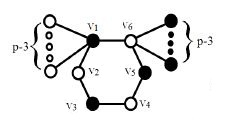
\includegraphics{sample2.jpg}
\end{center}
\caption{A Monocyclic Graph $C_6(p-3,p-3)$}
\label{fig:c6(p-3,p-3)}
\end{figure}

\begin{figure}[ht]
\begin{center}
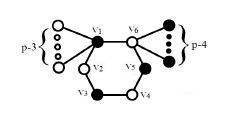
\includegraphics{sample3.jpg}
\end{center}
\caption{A Monocyclic Graph $C_6(p-3,p-4)$}
\label{fig:c6(p-3,p-4)}
\end{figure}

\begin{figure}[!ht]
\begin{center}
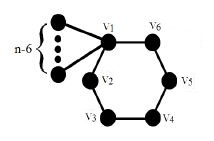
\includegraphics{sample4.jpg}
\end{center}
\caption{A Monocyclic Graph $C_6(n-6,0)$}
\label{fig:c6(n-6,0)}
\end{figure}

\begin{e.g.}\rm
Take $C_6(s,t)$ be a monocyclic graph with $C_6$ as its cycle, we now verify the results in \cite{wiener_ind_bipart} using Theorem \ref{thm:wiener_ckst}:
\begin{enumerate}
\item {$W(C_6(p-3,p-3))=5p^2-2p-12$, where $p\geq 4$.\\
Now, in figure \ref{fig:c6(p-3,p-3)}
$W(C_6(p-3,p-3))=\frac{1}{2}[2(p-3)^2+2(p-3)^2-2(p-3)-2(p-3)+6(p-3)(p-3)+9(2(p-3)+2(p-3)+6)+12(p-3)+12(p-3)]$, then we have $W(C_6(p-3,p-3))=\frac{1}{2}[10(p-3)^2+56(p-3)+54]$. Simply the results, we now have
$$
W(C_6(p-3,p-3))=\frac{1}{2}(10p^2-4p-24)=5p^2-2p-12
$$ 
and we are done.
}

\item {$W(C_6(p-3,p-4))=5p^2-7p-10$, where $p\geq 4$.\\
Now, in figure \ref{fig:c6(p-3,p-4)}
$W(C_6(p-3,p-4))=\frac{1}{2}[2(p-3)^2+2(p-4)^2-2(p-3)-2(p-4)+6(p-3)(p-4)+9(2(p-3)+2(p-4)+6)+12(p-3)+12(p-4)]$, then we have $W(C_6(p-3,p-4))=\frac{1}{2}[2(p-3)^2+2(p-4)^2+6(p-3)(p-4)+28(p-3)+28(p-4)+54]$. Simply the results, we now have
$$
W(C_6(p-3,p-4))=\frac{1}{2}(10p^2-14p-20)=5p^2-7p-10
$$ 
and we are done.}

\item {$W(C_6(n-6,0))=n^2+2n-21$, where $n\geq 6$.\\
Now, in figure \ref{fig:c6(n-6,0)}
$W(C_6(n-6,0))=\frac{1}{2}[2(n-6)^2+2(0)^2-2(n-6)-2(0)+6(n-6)(0)+9(2(n-6)+2(0)+6)+12(n-6)+12(0)]$, then we have $W(C_6(n-6,0))=\frac{1}{2}[2(n-6)^2+28(n-6)+54]$. Simply the results, we now have
$$
W(C_6(n-6,0))=\frac{1}{2}(2n^2-4n-42)=n^2-2n-21
$$ 
and we are done.}
\end{enumerate}
\end{e.g.}


\section{Zagreb Index of Monocyclic Graph $C_k(s,t)$}

\begin{thm}\rm
Suppose we partition the vertex set of monocyclic graph $C_k(s,t)$ into $G_s,G_k$ and $G_t$. Then the \textbf{Zagreb index} of $C_k(s,t)$ is
\begin{equation}
Zg(C_k(s,t))=s^2+t^2+8s+8t+4k
\label{eqn:zagreb}
\end{equation}
\label{thm:zagreb_mg} 
\end{thm}
\proof Given sets $G_s,G_k$, and $G_t$ wherein $V(C_k(s,t))=G_s\cup G_k\cup G_t$, it is evident that $|G_1|=s$, $|G_2|=k$, and $|G_3|=t$. Since, $deg(u)=2,\forall u\in G_s$, $deg(u)=2,\forall u \in G_t, deg(u)=2, \forall u \in G_k-{v_1,v_k} $, where $v_1$ and $v_2$ are the two adjacent vertices where \textbf{pendant vertices} $G_s$ and $G_t$ are attached respectively. Note that, $deg(v_1)=s+2$ and $deg(v_k)=t+2$. By definition \href{chap2.tex}{\ref{sec:m1(g)}} \textbf{Zagreb index} of monocyclic graph $C_k(s,t)$ is $Zg(C_k(s,t))=s(deg(u\in G_s))^2+t(deg(u\in G_t))^2+(s+2)^2+(t+2)^2+(k-2)(deg(u\in G_k-\left\lbrace v_1,v_k \right\rbrace))$. Simplifying further we have, $s(1^2)+t(1^2)+(s+2)^2+(t+2)^2+(k-1)(2^2)$ which is equal to $s^2+t^2+5s+5t+4k$. \medskip 

Thus, \textbf{Zagreb index} of $C_k(s,t)$ is $Zg(C_k(s,t))=s^2+t^2+5s+5t+4k$. \qed

\begin{e.g.}\rm
In figure \ref{fig:c4(2,3)}, the Zagreb index of the graph would be, $1^2+1^2+4^2+2^2+2^2+5^2+1^2+1^2+1^2=54$. Using equation \ref{eqn:zagreb} we have $Zg(C_4(2,3))=2^2+3^2+5(2)+5(3)+4(4)=54$.
\end{e.g.}

\begin{e.g.}\rm
In figure \ref{fig:c5(3,3)}, the Zagreb index of the graph would be, $1^2+1^2+1^2+5^2+2^2+2^2+2^2+5^2+1^2+1^2+1^2=68$. Using equation \ref{eqn:zagreb}, $Zg(C5(3,3))=3^2+3^2+5(3)+5(3)+4(5)=68$
\end{e.g.}

\section{Molecular Topological Index of Monocyclic Graph $C_k(s,t)$}
\begin{thm}\rm
Let $x\in V(C_k)$, then the Molecular Topological Index of monocyclic graph $C_k(s,t)$ is 
\begin{equation}
MTI(C_k(s,t))=4s^2+4t^2+6s+6t+10st+2w(x,C_k)(2s+2t+k)+3sk+3kt+4k 
\label{mti_ckst}
\end{equation}
where
$$
w(x,C_k)=\left\lbrace\begin{array}{cc}
\frac{k^2}{4} & $if k is even \\ 
\frac{(k+1)(k-1)}{4} & $if k is odd
\end{array}
$$
\label{thm:mti_mg}
\end{thm}

\proof
Using definition \href{chap2.tex}{\ref{sec:s_mti}}, we can now safely evaluate the \textbf{MTI} of the monocyclic graph $C_k(s,t)$.

Now that we calculated the degree distance index by Theorem \ref{thm:dd_mg} and the zagreb index using Theorem \ref{thm:zagreb_mg} by simple algebraic manipulation we arrived at Theorem \ref{thm:mti_mg}.
\qed

\begin{e.g.}\rm
In figure \ref{fig:c4(2,3)}, Degree distance index and Zagreb index are solved. Found that $DD(C_4(2,3))=261$ and $Zg(C_k(s,t))=54$. This would yield to an $MTI(C_4(2,3))=261+54=315$. Using Theorem \ref{thm:mti_mg}, $MTI(C_4(2,3))=4(2^2)+4(3^2)+3(2)+3(3)+10(2)(3)+2(4)(2(2)+2(3)+4)+3(2)(4)+3(4)(3)+4(4)=315$.
\end{e.g.}

\begin{e.g.}\rm
In figure \ref{fig:c5(3,3)}, Degree distance index and Zagreb index are already solved. The values are the following, $DD(C_5(3,3))=426$ and $Zg(C_5(3,3))=68$. Hence, $MTI(C_5(3,3))=426+68=494$. Using Theorem \ref{thm:mti_mg}, $MTI(C_5(3,3))=4(3^2)+4(3^2)+3(3)+3(3)+10(3)(3)+2(6)(2(3)+2(3)+5)+3(3)(5)+3(5)(3)+4(5)=494$.
\end{e.g.}

\begin{table}[!ht]
\caption{Degree Distance Index of $C_4(2,3)$ at $x$ by Inspection}
\begin{center}
\begin{tabular}{|c|c|c|c|c|}
\hline 
$x\in V(C_k(s,t))$ & $deg (x)$ & $w(x,C_k(s,t))$ & $dd(v_x,C_k(s,t))$  \\ 
\hline 
$x=v_1$ & 4 & 12 & 48 \\ 
\hline 
$x=v_4$ & 5 & 11 & 55 \\ 
\hline 
$x=v_2$ & 2 & 17 & 34 \\ 
\hline 
$x=v_3$ & 2 & 16 & 32 \\ 
\hline 
$x=u_1$ & 1 & 19 & 19 \\ 
\hline 
$x=u_2$ & 1 & 19 & 19 \\ 
\hline
$x=w_1$ & 1 & 18 & 18 \\ 
\hline 
$x=w_2$ & 1 & 18 & 18 \\ 
\hline 
$x=w_3$ & 1 & 18 & 18 \\ 
\hline 
$TOTAL$ & 18 & 148 & 261 \\ 
\hline 
\end{tabular} 
\end{center}
\label{tab:DD_c4_inspection}
\end{table}

\newpage
\begin{table}[!ht]
\caption{Degree Distance Index of $C_5(3,3)$ at $x$ by Inspection}
\begin{center}
\begin{tabular}{|c|c|c|c|c|}
\hline 
$x\in V(C_k(s,t))$ & $deg (x)$ & $w(x,C_k(s,t))$ & $dd(v_x,C_k(s,t))$  \\ 
\hline 
$x=v_1$ & 5 & 15 & 75 \\ 
\hline 
$x=v_5$ & 5 & 15 & 75 \\ 
\hline 
$x=v_2$ & 2 & 21 & 42 \\ 
\hline 
$x=v_3$ & 2 & 24 & 48 \\ 
\hline 
$x=v_3$ & 2 & 21 & 42 \\ 
\hline 
$x=u_1$ & 1 & 24 & 24 \\ 
\hline 
$x=u_2$ & 1 & 24 & 24 \\ 
\hline 
$x=w_1$ & 1 & 18 & 18 \\ 
\hline
$x=u_3$ & 1 & 24 & 24 \\ 
\hline  
$x=w_2$ & 1 & 18 & 18 \\ 
\hline 
$x=w_1$ & 1 & 24 & 24 \\ 
\hline 
$x=w_2$ & 1 & 24 & 24 \\ 
\hline 
$x=w_3$ & 1 & 24 & 24 \\ 
\hline 
$TOTAL$ & 22 & 240 & 426 \\ 
\hline 
\end{tabular} 
\end{center}
\label{tab:DD_c4_inspection}
\end{table}

\begin{table}[!ht]
\caption{Molecular Topological Index of Some Monocyclic Graph $C_k(s,t)$}
\begin{center}
\begin{tabular}{|c|c|c|c|c|c|}
\hline 
$k-cycles$ & $s$ & $t$ & $DD(C_k(s,t))$ & $Zg(C_k(s,t))$ & $MTI$ \\  
\hline 
$4$ & 2 & 3 & 261 & 69 & 330 \\ 
\hline 
$4$ & 3 & 3 & 332 & 82 & 414 \\ 
\hline 
$4$ & 5 & 5 & 692 & 146 & 838 \\ 
\hline 
$5$ & 2 & 3 & 344 & 73 & 417 \\ 
\hline 
$5$ & 4 & 4 & 612 & 116 & 728 \\ 
\hline 
$5$ & 10 & 10 & 2400 & 380 & 2780 \\ 
\hline
\end{tabular} 
\end{center}
\label{tab:mti_some_mg}
\end{table}



